\chapter{Empreendedorismo Corporativo, Intraempreendedorismo e \textit{Spin-offs}}
\label{cap:11}
\markboth{CAPÍTULO 11: INTRAEMPREENDEDORISMO E SPIN-OFFS}{CAPÍTULO 11: INTRAEMPREENDEDORISMO E SPIN-OFFS}

\noindent\tagAV{Base AV3}

\begin{capObjetivos}
  Ao concluir este capítulo, você será capaz de:
  \begin{enumerate}[leftmargin=1.5em, itemsep=2pt]
    \item Distinguir \textbf{intraempreendedorismo} (\textit{Pinchot, 1985}) e \textbf{empreendedorismo corporativo} (\textit{Guth \& Ginsberg, 1990}) como estratégias de renovação e criação de novos negócios em organizações existentes.
    \item Analisar fluxos de \textbf{\textit{Open Innovation}} (\textit{Chesbrough}) nas vertentes \textit{inbound} (incorporação externa) e \textit{outbound} (externalização e licenciamento).
    \item Modelar a criação de \textbf{\textit{spin-offs} acadêmicas} na transição ICT/NIT para o mercado, calculando taxas de \textit{royalties} e repartição de ganhos econômicos sob o Marco Legal de CT\&I (\textbf{Lei nº 13.243/2016}).
    \item Aplicar o conceito de \textbf{intraempreendedorismo público} e instrumentos como a Encomenda Tecnológica (ETEC) ao planejamento territorial.
  \end{enumerate}
\end{capObjetivos}

\begin{capRevisao}
  Conecte os temas deste capítulo ao percurso da Unidade II:
  \begin{itemize}[leftmargin=1.5em, itemsep=2pt]
    \item \textbf{Vale da Morte e TRL (Cap. 7):} o licenciamento de tecnologias já validadas em ICTs ou corporações reduz o tempo de travessia até o mercado.
    \item \textbf{Propriedade Intelectual (Cap. 8):} a transferência de tecnologia em \textit{spin-offs} e inovação aberta depende de ativos protegidos (patentes, software, cultivares) e de contratos de FTO.
    \item \textbf{Escada do Capital (Cap. 10):} \textit{spin-offs} e projetos de intraempreendedorismo podem combinar orçamento corporativo/público com fomento da FINEP, FAPs e crédito regional.
  \end{itemize}
\end{capRevisao}

\etapa{3}{Explicação Teórica, Vocabulário Prévio e Modelos}

\begin{boxSimbolo}[Vocabulário Conceitual e Símbolos do Capítulo 11]
  \begin{tabularx}{\textwidth}{@{}l >{\raggedright\arraybackslash}X@{}}
    \textbf{Intraempreendedor} & Colaborador que atua com autonomia empreendedora dentro de uma organização privada ou pública para criar novos produtos, serviços ou processos. \\
    \textbf{\textit{Open Innovation}} & Paradigma em que empresas usam fluxos internos e externos de conhecimento para acelerar a inovação e ampliar mercados. \\
    \textbf{\textit{Inbound} / \textit{Outbound}} & \textit{Inbound}: absorção de tecnologias externas pela empresa; \textit{Outbound}: licenciamento ou \textit{spin-out} de tecnologias internas ociosas. \\
    \textbf{ICT / NIT} & Instituição Científica, Tecnológica e de Inovação (universidades/institutos) e seu Núcleo de Inovação Tecnológica. \\
    \textbf{\textit{Spin-off} Acadêmica} & Nova empresa constituída para explorar comercialmente conhecimento ou PI gerados no âmbito de uma ICT. \\
    \textbf{$R_{\text{roy}}$, $r$, $\alpha_{\text{inv}}$} & Receita anual de \textit{royalties}, alíquota contratual sobre faturamento líquido e parcela destinada aos inventores (art. 13 da Lei de Inovação). \\
  \end{tabularx}
\end{boxSimbolo}

\section{Inovar Sem Começar do Zero: Intraempreendedorismo e Empreendedorismo Corporativo}

A criação de valor tecnológico ocorre tanto em startups independentes quanto no interior de organizações já estabelecidas. Organizações consolidadas (empresas industriais, cooperativas agropecuárias, hospitais e órgãos públicos) detêm ativos complementares valiosos, como canais de distribuição, base de clientes, infraestrutura laboratorial e marca, mas frequentemente sofrem de inércia burocrática.

Em 1985, Gifford Pinchot cunhou o termo \textbf{intraempreendedorismo} (\textit{intrapreneurship}) para descrever o comportamento de profissionais que assumem responsabilidade direta por transformar ideias em inovações rentáveis dentro das fronteiras da organização empregadora. Enquanto o intraempreendedorismo foca o nível individual ou de equipe, William Guth e Ari Ginsberg (1990) formalizaram o **empreendedorismo corporativo** no nível estratégico da firma, abrangendo duas dimensões complementares: o **\textit{corporate venturing}** (criação de novos negócios internos ou *spin-outs* dentro ou fora da empresa-mãe) e a **renovação estratégica** (reconfiguração do modelo de negócio e das competências centrais para responder a mudanças ambientais).

\section{\textit{Open Innovation}: Fluxos \textit{Inbound} e \textit{Outbound} (Chesbrough)}

No modelo fechado tradicional de P\&D, grandes corporações mantinham laboratórios isolados, acreditando que apenas a pesquisa própria garantia qualidade e apropriação. Henry Chesbrough (2003) indicou que a mobilidade de talentos e a dispersão global do conhecimento tornaram esse modelo lento e oneroso, propondo a **Inovação Aberta (\textit{Open Innovation})**.

A inovação aberta opera em duas direções estratégicas complementares que conectam a empresa ao ecossistema territorial. No fluxo \textbf{\textit{Open Innovation Inbound} (de fora para dentro)}, a organização incorpora tecnologias, patentes ou soluções desenvolvidas por universidades, startups ou fornecedores externos, reduzindo o tempo de desenvolvimento e o risco técnico, como ocorre quando uma indústria alimentícia regional licencia um biofilme conservante desenvolvido por uma universidade estadual. No sentido oposto, o fluxo \textbf{\textit{Open Innovation Outbound} (de dentro para fora)} permite que a organização identifique tecnologias geradas internamente que escapam ao seu negócio central (\textit{core business}) e as monetize por meio de licenciamento para terceiros, venda de patentes ou criação de uma nova empresa (\textit{spin-out}).

\section{\textit{Spin-offs} Acadêmicas e o Marco Legal de CT\&I (Lei nº 13.243/2016)}

Uma **\textit{spin-off} acadêmica** é uma empresa nascente originada a partir de pesquisas, competências ou Propriedade Intelectual geradas dentro de uma Instituição Científica, Tecnológica e de Inovação (ICT). No Brasil, a relação entre universidade e empresa foi profundamente modernizada pela **Lei nº 13.243/2016** (Marco Legal de Ciência, Tecnologia e Inovação), que alterou a Lei de Inovação (Lei nº 10.973/2004) e foi regulamentada pelo Decreto nº 9.283/2018.

Esse marco legal instituiu mecanismos específicos para destravar *spin-offs* e parcerias territoriais. Os **Núcleos de Inovação Tecnológica (NITs)** passaram a gerir a política de PI da ICT, apoiando a proteção patentária e negociando contratos de transferência de tecnologia e licenciamento, com possibilidade inclusive de constituírem personalidade jurídica própria por meio de fundações de apoio ou associações. Além disso, a legislação autoriza o **compartilhamento de laboratórios e infraestrutura**, permitindo que a ICT ceda o uso de equipamentos e capital intelectual a empresas e startups mediante contrapartida financeira ou não financeira, o que reduz o CAPEX inicial na fase TRL 3–6. No plano da governança de pessoas, o pesquisador público em regime de dedicação exclusiva pode afastar-se ou atuar em atividades de pesquisa e participação societária em *spin-offs* conforme regulamentação da ICT, além de receber bolsa de estímulo à inovação. Para alinhar incentivos econômicos, o art. 13 da Lei nº 10.973/2004 assegura aos criadores (inventores) **participação nos ganhos econômicos (\textit{royalties})** situada entre o mínimo de **5\%** e o máximo de **1/3 (33{,}33\%)** dos valores auferidos pela ICT com o licenciamento ou cessão da criação protegida.

\section{Intraempreendedorismo Público no Planejamento Territorial}

O intraempreendedorismo estende-se também à esfera governamental e comunitária. No setor público (prefeituras, consórcios intermunicipais, secretarias estaduais e agências de desenvolvimento), servidores intraempreendedores mobilizam compras públicas, laboratórios de governo e parcerias com ICTs para resolver gargalos territoriais. O Marco Legal de CT\&I autoriza instrumentos como a **Encomenda Tecnológica (ETEC)** (art. 20), que permite à administração pública contratar diretamente ICTs ou empresas para desenvolver soluções com risco tecnológico inédito em benefício do território, como sistemas de monitoramento de secas, saneamento rural ou gestão de resíduos. A articulação entre fluxos de inovação aberta, transferência tecnológica via NIT e emergência de *spin-offs* acadêmicas rumo ao mercado sob a Lei nº 13.243/2016 está sintetizada na Figura~\ref{fig:11_open_innovation_spinoff}.

\begin{figure}[H]
  \centering
  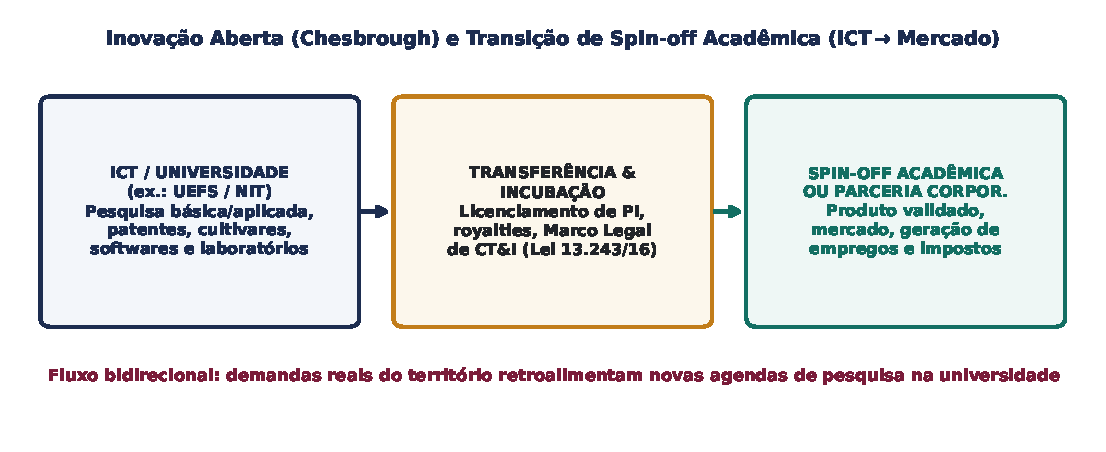
\includegraphics[width=0.94\textwidth]{figures/fig11_open_innovation_spinoff.pdf}
  \caption{Fluxos de \textit{Open Innovation} (\textit{inbound} e \textit{outbound}) e transição de \textit{spin-off} acadêmica da ICT/NIT para o mercado sob a Lei nº 13.243/2016.}
  \label{fig:11_open_innovation_spinoff}
\end{figure}

\begin{boxFormula}[Cálculo de \textit{Royalties} e Repartição Legal em Licenciamento de ICT (Lei 13.243/2016)]
  Considere uma \textit{spin-off} acadêmica (ou empresa licenciada) que comercializa um produto baseado em tecnologia protegida da ICT, obtendo faturamento líquido anual $F_{\text{líq}}$ (receita bruta deduzida de impostos sobre vendas e devoluções). Sendo $r$ a taxa contratual de \textit{royalty} (em decimal), a receita anual de licenciamento paga à ICT é:
  \[
    R_{\text{roy}} = F_{\text{líq}} \times r.
  \]
  De acordo com o art. 13 da Lei nº 10.973/2004 (atualizada pela Lei nº 13.243/2016), a parcela destinada aos criadores/inventores ($\alpha_{\text{inv}}$) deve situar-se no intervalo $0{,}05 \le \alpha_{\text{inv}} \le \frac{1}{3}$ (entre $5\%$ e $33{,}33\%$). Assim:
  \[
    G_{\text{inventores}} = R_{\text{roy}} \times \alpha_{\text{inv}}, \qquad
    G_{\text{ICT/NIT}} = R_{\text{roy}} \times (1 - \alpha_{\text{inv}}).
  \]
  Se houver $k$ inventores com participação igualitária na criação, cada inventor recebe $G_{\text{inventores}} / k$.
\end{boxFormula}

\etapa{4}{Estudos de Caso e Exemplos Resolvidos em 7 Passos}

\begin{boxExemplo}{11.1}{Licenciamento e Repartição de \textit{Royalties} em \textit{Spin-off} da UEFS}
  \passoEnunciado{Uma \textit{spin-off} fundada por egressos do PPGPT/UEFS licenciou junto ao NIT da universidade uma patente de sensor de umidade do solo de baixo custo.}
  \passoDados{Faturamento líquido anual da \textit{spin-off} com o sensor licenciado: $F_{\text{líq}} = \text{R\$\,1.200.000,00}$. Alíquota contratual de \textit{royalty}: $r = 4\%$ ($0{,}04$) sobre o faturamento líquido. Política de inovação da ICT: destina o teto legal de $\alpha_{\text{inv}} = 1/3$ ($33{,}33\%$) aos criadores (equipe de 2 inventores com partes iguais) e $2/3$ ($66{,}67\%$) à ICT/laboratório/NIT.}
  \passoPedido{Calcular o valor anual total de \textit{royalties} transferido à ICT, a parcela total dos inventores, o ganho individual de cada inventor e a parcela retida pela ICT/NIT.}
  \passoMetodo{Aplicação das equações de licenciamento e repartição conforme o art. 13 da Lei de Inovação.}
  \passoContas{
    Primeiro, calcula-se a receita total anual de \textit{royalties}:
    \[
      R_{\text{roy}} = 1.200.000,00 \times 0{,}04 = \text{R\$\,48.000,00/ano}.
    \]
    Em seguida, realiza-se a repartição entre os inventores ($1/3$) e a ICT/NIT ($2/3$):
    \[
      G_{\text{inventores}} = 48.000,00 \times \frac{1}{3} = \text{R\$\,16.000,00/ano},
    \]
    \[
      G_{\text{ICT/NIT}} = 48.000,00 \times \frac{2}{3} = \text{R\$\,32.000,00/ano}.
    \]
    Como há 2 inventores com participação igualitária, cada um recebe:
    \[
      G_{\text{por inventor}} = \frac{16.000,00}{2} = \text{R\$\,8.000,00/ano}.
    \]
  }
  \passoResposta{\textit{Royalties} totais $= \text{R\$\,48.000,00/ano}$; inventores $= \text{R\$\,16.000,00/ano}$ (R\$\,8.000,00 cada); ICT/NIT $= \text{R\$\,32.000,00/ano}$.}
  \passoVerificacao{Uma alíquota de 4\% sobre o faturamento líquido preserva a margem operacional da \textit{spin-off} enquanto gera retorno contínuo para retroalimentar o laboratório de origem.}
\end{boxExemplo}

\begin{boxExemplo}{11.2}{\textit{Open Innovation Inbound}: Licenciamento vs. P\&D Interno}
  \passoEnunciado{Uma indústria média de beneficiamento de couro e curtume no polo industrial de Feira de Santana precisa implantar um sistema de tratamento biológico de efluentes para atender à fiscalização ambiental.}
  \passoDados{Opção 1 (P\&D Interno fechado): investimento inicial de R\$\,600.000,00, prazo de desenvolvimento de 24 meses e custo de oportunidade por atraso de adequação ambiental de R\$\,15.000,00/mês. Opção 2 (\textit{Open Innovation Inbound}): licenciar tecnologia TRL 6 de uma ICT regional com taxa de adaptação de R\$\,180.000,00, prazo de 8 meses e pagamento fixo anual de licença de R\$\,36.000,00.}
  \passoPedido{Calcular a economia de CAPEX inicial, o ganho de tempo até a operação e o custo evitado de atraso na Opção 2.}
  \passoMetodo{Análise comparativa entre desenvolvimento fechado (\textit{make}) e incorporação aberta (\textit{buy/license}).}
  \passoContas{
    Economia de desembolso inicial (CAPEX de P\&D):
    \[
      \Delta \text{CAPEX} = 600.000,00 - 180.000,00 = \text{R\$\,420.000,00} \quad \left(\frac{420.000}{600.000} = 70{,}0\%\text{ de redução}\right).
    \]
    Ganho de tempo até a implantação: $24 - 8 = 16\text{ meses}$.
    Economia com custos evitados de atraso ambiental durante esses 16 meses:
    \[
      \text{Economia de atraso} = 16 \times 15.000,00 = \text{R\$\,240.000,00}.
    \]
    Mesmo pagando R\$\,36.000,00/ano de licença, os R\$\,420.000,00 economizados na entrada cobririam mais de 11 anos de anuidade de licenciamento.
  }
  \passoResposta{A estratégia \textit{inbound} reduz o CAPEX inicial em 70{,}0\% (R\$\,420.000,00), antecipa a operação em 16 meses e evita R\$\,240.000,00 em custos de atraso.}
  \passoVerificacao{O resultado explica por que médias empresas regionais sem laboratório próprio obtêm maior retorno adotando inovação aberta junto a ICTs.}
\end{boxExemplo}

\begin{boxExemplo}{11.3}{Empreendedorismo Corporativo e Renovação em Cooperativa Agroindustrial}
  \passoEnunciado{Uma cooperativa de processamento de mandioca observa queda de margem na venda de fécula comum e analisa uma proposta interna de dois engenheiros colaboradores para criar uma unidade de biogás e bioenergia a partir da manipueira (resíduo líquido tóxico do processamento).}
  \passoDados{Custo atual de descarte e tratamento da manipueira em lagoas: R\$\,14.000,00/mês. Investimento corporativo interno na planta de biodigestão: R\$\,480.000,00. Economia mensal de energia elétrica gerada pelo biogás: R\$\,16.000,00/mês (além de eliminar os R\$\,14.000,00/mês de custo de descarte).}
  \passoPedido{Classificar a iniciativa segundo Pinchot (1985) e Guth \& Ginsberg (1990) e calcular o ganho econômico mensal total e o \textit{payback} simples da unidade interna.}
  \passoMetodo{Identificação de intraempreendedorismo/renovação estratégica e cálculo de retorno sobre economia operacional.}
  \passoContas{
    Trata-se de \textbf{intraempreendedorismo} liderado pelos dois engenheiros e de \textbf{empreendedorismo corporativo} (criação de unidade interna de negócio e renovação ambiental da cooperativa).
    O benefício econômico mensal total soma a eliminação do custo de descarte e a economia de energia:
    \[
      \text{Benefício mensal} = 14.000,00 + 16.000,00 = \text{R\$\,30.000,00/mês}.
    \]
    O \textit{payback} simples do investimento corporativo de R\$\,480.000,00 é:
    \[
      \text{Payback} = \frac{480.000,00}{30.000,00} = 16\text{ meses}.
    \]
  }
  \passoResposta{A iniciativa gera benefício econômico de R\$\,30.000,00/mês e retorna o capital corporativo em 16 meses, convertendo um passivo ambiental em ativo energético.}
  \passoVerificacao{A infraestrutura já existente da cooperativa (fluxo garantido de manipueira e demanda própria de energia) elimina o risco comercial que uma startup independente enfrentaria.}
\end{boxExemplo}

\begin{boxExemplo}{11.4}{\textit{Open Innovation Outbound}: Monetização de Tecnologia Não Central}
  \passoEnunciado{Uma empresa de logística agrícola desenvolveu internamente um algoritmo de roteirização para estradas vicinais não pavimentadas do interior baiano. Como seu negócio principal é transporte de cargas próprias e não venda de software, o algoritmo atendia apenas à frota interna.}
  \passoDados{Custo adicional para empacotar a API para terceiros (\textit{outbound}): R\$\,45.000,00. Contrato de licenciamento não exclusivo para 15 cooperativas regionais a R\$\,1.500,00/mês por cooperativa.}
  \passoPedido{Calcular a receita anual bruta gerada pelo fluxo \textit{outbound} e em quantos meses o investimento de empacotamento é recuperado.}
  \passoMetodo{Análise de monetização de ativos ociosos via \textit{Open Innovation Outbound}.}
  \passoContas{
    Receita mensal do licenciamento para 15 cooperativas:
    \[
      R_{\text{mensal}} = 15 \times 1.500,00 = \text{R\$\,22.500,00/mês}.
    \]
    Receita anual bruta:
    \[
      R_{\text{anual}} = 22.500,00 \times 12 = \text{R\$\,270.000,00/ano}.
    \]
    Tempo para recuperar o custo de empacotamento da API (R\$\,45.000,00):
    \[
      \text{Payback} = \frac{45.000,00}{22.500,00} = 2{,}0\text{ meses}.
    \]
  }
  \passoResposta{O licenciamento \textit{outbound} gera R\$\,270.000,00/ano de nova receita com recuperação do custo de adaptação em apenas 2 meses.}
  \passoVerificacao{Em vez de deixar o ativo subutilizado dentro da firma ou tentar virar uma empresa de software concorrente do próprio negócio, a estratégia \textit{outbound} gera receita de alta margem.}
\end{boxExemplo}

\begin{boxExemplo}{11.5}{Intraempreendedorismo Público e Encomenda Tecnológica (ETEC)}
  \passoEnunciado{Um consórcio intermunicipal do Semiárido enfrenta recorrentes perdas de água em cisternas comunitárias por falta de detecção precoce de fissuras e contaminação microbiológica, sem encontrar solução comercial pronta no mercado para regiões sem cobertura celular.}
  \passoDados{Orçamento disponível para compras de emergência com caminhões-pipa: R\$\,900.000,00/ano. Uma servidora intraempreendedora propõe estruturar uma Encomenda Tecnológica (ETEC, art. 20 da Lei nº 10.973/2004) junto a uma ICT regional e uma startup local por R\$\,320.000,00 em 12 meses para desenvolver sensores autônomos via rádio LoRa.}
  \passoPedido{Explicar por que a licitação tradicional de menor preço falharia nesse caso e calcular a economia potencial se o sistema reduzir em 30\% o gasto anual com caminhões-pipa após implantado.}
  \passoMetodo{Aplicação do regime jurídico de ETEC (risco tecnológico) e estimativa de benefício fiscal territorial.}
  \passoContas{
    A licitação comum exige especificações técnicas já existentes no mercado; como há risco tecnológico inédito (sensores de baixo custo sem rede celular), a ETEC é o instrumento legal adequado.
    Se a solução reduzir em 30\% o gasto anual de R\$\,900.000,00 com caminhões-pipa, a economia anual será:
    \[
      \text{Economia anual} = 900.000,00 \times 0{,}30 = \text{R\$\,270.000,00/ano}.
    \]
    Comparando com o valor da ETEC (R\$\,320.000,00), o investimento público paga-se em $320.000 / 270.000 \approx 1{,}19\text{ ano}$ (cerca de 14{,}2 meses de operação).
  }
  \passoResposta{A ETEC viabiliza contratação pública sob risco tecnológico; a economia estimada de R\$\,270.000,00/ano recupera o investimento público em 1{,}19 ano.}
  \passoVerificacao{O intraempreendedorismo público transforma o poder de compra do Estado em motor de desenvolvimento tecnológico territorial.}
\end{boxExemplo}

\etapa{5}{Armadilhas Conceituais e Erros Mais Comuns}

\begin{boxErro}[Erro 1: Confundir \textit{Spin-off} Acadêmica com Projeto de Extensão sem Modelo de Negócio]
  Muitas equipes universitárias registram um CNPJ formal mantendo a lógica acadêmica de dependência exclusiva de bolsas, sem definir clientes pagantes, preços ou governança societária. Uma \textit{spin-off} exige separação clara entre a pesquisa acadêmica da ICT e a operação comercial autônoma da empresa.
\end{boxErro}

\begin{boxErro}[Erro 2: Fixar Taxas de \textit{Royalties} Proibitivas no Contrato com o NIT]
  Exigir \textit{royalties} elevados logo nos primeiros meses (ou pagamentos mínimos anuais desconectados da receita) inviabiliza a sobrevivência da \textit{spin-off} durante o Vale da Morte. A prática moderna adota taxas escalonadas ou vinculadas ao faturamento líquido após o início das vendas comerciais.
\end{boxErro}

\begin{boxErro}[Erro 3: Promover Intraempreendedorismo sem Autonomia nem Proteção contra Falhas]
  Pedir inovação aos colaboradores enquanto se pune qualquer experimento malsucedido com sanções na carreira destrói o intraempreendedorismo. Organizações precisam criar espaços protegidos de experimentação com métricas de aprendizado e perda aceitável definida.
\end{boxErro}

\begin{boxErro}[Erro 4: Tratar \textit{Open Innovation} como Terceirização Simples de Serviços]
  Contratar uma empresa de TI para executar um escopo fechado não é \textit{Open Innovation}. A inovação aberta envolve compartilhamento genuíno de risco, conhecimento tecnológico e propriedade intelectual entre parceiros externos e internos.
\end{boxErro}

\etapa{6}{Lista de Exercícios (15 Questões em 3 Níveis)}

\textbf{Nível 1, Fundamentos Conceituais (Questões 1 a 5)}

\begin{enumerate}[leftmargin=1.5em, itemsep=6pt]
  \item Diferencie intraempreendedorismo (Pinchot, 1985) de empreendedorismo corporativo (Guth \& Ginsberg, 1990) quanto ao nível de análise e aos resultados esperados na organização.
  \espacoResolucao[1.8cm]

  \item Explique a diferença entre \textit{Open Innovation Inbound} e \textit{Open Innovation Outbound}, citando um exemplo territorial para cada fluxo.
  \espacoResolucao[1.8cm]

  \item Qual é o papel do Núcleo de Inovação Tecnológica (NIT) na criação de uma \textit{spin-off} acadêmica sob a Lei nº 13.243/2016?
  \espacoResolucao[1.8cm]

  \item Cite três instrumentos previstos no Marco Legal de CT\&I (Lei nº 13.243/2016) que facilitam a transição da pesquisa universitária para o setor produtivo.
  \espacoResolucao[1.8cm]

  \item O que caracteriza o intraempreendedorismo público e em que situações a Encomenda Tecnológica (ETEC) substitui a licitação tradicional?
  \espacoResolucao[1.8cm]

  \item \textbf{(Nível 2, Aplicações Numéricas)} Uma \textit{spin-off} faturou R\$\,800.000,00 líquidos no ano com um produto licenciado de uma universidade pública, sob alíquota de \textit{royalty} de 5\%. Sabendo que a ICT destina 25\% dos ganhos aos inventores, calcule o total de \textit{royalties} pagos pela empresa, o valor recebido pelos inventores e o valor retido pela ICT/NIT.
  \espacoResolucao[2.3cm]

  \item No exercício anterior, se o pedido de patente teve 4 inventores com participação igualitária, quanto cada inventor recebeu no ano?
  \espacoResolucao[2.0cm]

  \item Uma cooperativa agroindustrial avalia duas opções para implantar rastreabilidade por QR Code: desenvolver internamente por R\$\,220.000,00 em 14 meses ou licenciar uma solução externa (\textit{inbound}) com implantação de R\$\,55.000,00 em 3 meses. Qual a economia percentual de desembolso inicial e quantos meses foram economizados?
  \espacoResolucao[2.2cm]

  \item Uma empresa licenciou em fluxo \textit{outbound} uma tecnologia não central para 8 empresas parceiras, cobrando taxa fixa de R\$\,2.500,00/mês por empresa. Sabendo que o custo anual de suporte técnico às licenciadas é de R\$\,40.000,00, qual é o ganho líquido anual gerado pelo licenciamento?
  \espacoResolucao[2.2cm]

  \item Um projeto de intraempreendedorismo em uma indústria têxtil exigiu R\$\,300.000,00 de investimento interno e passou a gerar economia mensal de água e insumos químicos de R\$\,25.000,00. Qual é o \textit{payback} simples desse projeto interno em meses?
  \espacoResolucao[2.1cm]

  \item \textbf{(Nível 3, Análise Territorial e Estratégica)} Analise por que uma \textit{spin-off} instalada em um município interiorano se beneficia mais do compartilhamento de laboratórios da ICT previsto na Lei nº 13.243/2016 do que da aquisição imediata de equipamentos próprios.
  \espacoResolucao[2.2cm]

  \item Uma universidade e uma \textit{spin-off} negociam contrato de licenciamento de patente. A \textit{spin-off} projeta faturamento líquido de R\$\,500.000,00 no Ano 1 e R\$\,1.500.000,00 no Ano 2. Compare dois modelos de cobrança pela ICT: Modelo A = taxa fixa anual de R\$\,60.000,00 desde o Ano 1; Modelo B = \textit{royalty} variável de 4\% sobre o faturamento líquido. Qual modelo protege melhor a \textit{spin-off} no Ano 1 e qual gera maior retorno acumulado para a ICT ao final dos 2 anos?
  \espacoResolucao[2.5cm]

  \item Discuta os principais conflitos de interesse que podem surgir quando um docente ou pesquisador público participa simultaneamente da ICT e de uma \textit{spin-off} acadêmica, e indique como a governança do NIT deve mitigá-los.
  \espacoResolucao[2.2cm]

  \item Uma prefeitura gasta R\$\,1.200.000,00/ano com coleta e destinação ineficiente de resíduos orgânicos de feiras livres. Um servidor intraempreendedor propõe uma ETEC de R\$\,240.000,00 com um instituto tecnológico para desenvolver biodigestor modular que reduza em 25\% o custo anual de destinação. Qual será a economia anual após a implantação e em quantos meses o investimento público se paga?
  \espacoResolucao[2.4cm]

  \item Elabore um fluxograma textual de 5 etapas mostrando como uma tecnologia protegida por uma ICT baiana percorre o caminho da bancada até o mercado via \textit{spin-off} acadêmica.
  \espacoResolucao[2.3cm]
\end{enumerate}

\etapa{7}{Questões Autorais Estilo Pós-Graduação / Concursos de CT\&I}

\begin{enumerate}[leftmargin=1.5em, itemsep=6pt]
  \item \textbf{(Estilo ANPAD / Gestão da Inovação)} Sobre inovação aberta (\textit{Open Innovation}) e empreendedorismo corporativo, assinale a alternativa correta:
  \begin{alternativas}
    \item O fluxo \textit{outbound} ocorre quando uma empresa adquire startups externas para substituir seu departamento de vendas.
    \item O empreendedorismo corporativo, segundo Guth e Ginsberg (1990), limita-se à criação de programas de sugestões de baixo custo sem impacto na estratégia da empresa.
    \item O fluxo \textit{inbound} permite à empresa absorver tecnologias externas desenvolvidas por ICTs ou startups, reduzindo tempo de desenvolvimento e risco técnico.
    \item Na inovação fechada, as empresas priorizam o licenciamento de patentes ociosas para concorrentes regionais.
    \item O intraempreendedorismo exige obrigatoriamente que o colaborador peça demissão para fundar uma empresa independente.
  \end{alternativas}
  \espacoResolucao[1.5cm]

  \item \textbf{(Estilo Concurso Gestor de CT\&I / NIT)} Uma ICT licenciou patente de bioinsumo para uma \textit{spin-off} sob taxa de \textit{royalty} de 3\% sobre o faturamento líquido. No exercício anual, a \textit{spin-off} faturou R\$\,2.000.000,00 líquidos. Sabendo que a política de inovação da ICT fixa a participação dos inventores no limite máximo permitido pela Lei nº 10.973/2004 (1/3 dos ganhos econômicos), o valor destinado aos inventores e o valor retido pela ICT são, respectivamente:
  \begin{alternativas}
    \item R\$\,3.000,00 e R\$\,57.000,00.
    \item R\$\,20.000,00 e R\$\,40.000,00.
    \item R\$\,15.000,00 e R\$\,45.000,00.
    \item R\$\,30.000,00 e R\$\,30.000,00.
    \item R\$\,60.000,00 e R\$\,120.000,00.
  \end{alternativas}
  \espacoResolucao[1.6cm]

  \item \textbf{(Estilo Discursiva, PPGPT)} Explique como o intraempreendedorismo público e a Encomenda Tecnológica (ETEC) previstos no Marco Legal de CT\&I podem atuar como indutores de sistemas locais de inovação em municípios de pequeno e médio porte.
  \espacoResolucao[2.3cm]
\end{enumerate}

\begin{boxDica}[Contraponto Crítico e Prática Territorial (AV3)]
  Se o seu Projeto Final (AV3) nasce de uma pesquisa de laboratório (ICT/UEFS) ou ocorre dentro de uma cooperativa/órgão público, explicite na seção estratégica qual é o regime de transferência tecnológica (licenciamento via NIT, compartilhamento de laboratório, *spin-off* ou intraempreendedorismo) e apresente o cálculo de *royalties* ou economia operacional esperado.
\end{boxDica}

\clearpage
\etapa{8}{Gabarito Integralmente Comentado (Exercícios 1 a 18)}

\begin{boxGabarito}[Resolução Completa dos Exercícios da Etapa 6 (1 a 15) e Etapa 7 (16 a 18)]
  \begin{enumerate}[leftmargin=1.5em, itemsep=4pt]
    \item \textbf{Resposta:} Intraempreendedorismo (Pinchot) foca a ação empreendedora de colaboradores dentro da organização; empreendedorismo corporativo (Guth \& Ginsberg) foca o nível estratégico da firma via criação de novos negócios (\textit{corporate venturing}) e renovação estratégica.
    \item \textbf{Resposta:} \textit{Inbound} é trazer tecnologia externa para dentro (ex.: indústria local licenciando biofilme de universidade); \textit{Outbound} é levar tecnologia interna para fora (ex.: empresa de logística licenciando algoritmo ocioso para cooperativas).
    \item \textbf{Resposta:} O NIT protege a PI da ICT, realiza busca de anterioridade, negocia contratos de transferência de tecnologia e licenciamento, e orienta a formalização da relação entre ICT e \textit{spin-off}.
    \item \textbf{Resposta:} Compartilhamento de laboratórios/infraestrutura da ICT com empresas; participação dos criadores em 5\% a 1/3 dos ganhos econômicos; Encomenda Tecnológica (ETEC) pelo poder público.
    \item \textbf{Resposta:} Intraempreendedorismo público é a inovação liderada por servidores dentro da administração pública. A ETEC substitui a licitação tradicional quando a solução desejada ainda não existe no mercado e envolve risco tecnológico inédito.
    \item \textbf{Resposta:} $R_{\text{roy}} = 800.000 \times 0{,}05 = \text{R\$\,40.000,00/ano}$. Parcela dos inventores $= 40.000 \times 0{,}25 = \text{R\$\,10.000,00/ano}$. Parcela da ICT/NIT $= 40.000 - 10.000 = \text{R\$\,30.000,00/ano}$.
    \item \textbf{Resposta:} Cada inventor recebeu $10.000,00 / 4 = \text{R\$\,2.500,00/ano}$.
    \item \textbf{Resposta:} Economia $= 220.000 - 55.000 = \text{R\$\,165.000,00}$, o que equivale a $165.000 / 220.000 = 75{,}0\%$ de redução no desembolso inicial. Economia de tempo $= 14 - 3 = 11\text{ meses}$.
    \item \textbf{Resposta:} Receita bruta anual $= 8 \times 2.500 \times 12 = \text{R\$\,240.000,00/ano}$. Ganho líquido anual $= 240.000 - 40.000 = \text{R\$\,200.000,00/ano}$.
    \item \textbf{Resposta:} $\text{Payback} = 300.000 / 25.000 = 12\text{ meses}$.
    \item \textbf{Resposta:} Porque reduz drasticamente o CAPEX inicial na fase TRL 3–6, evitando que a \textit{spin-off} imobilize capital escasso em equipamentos analíticos caros antes de validar vendas recorrentes no território.
    \item \textbf{Resposta:} Modelo A (fixo): Ano 1 = R\$\,60.000; Ano 2 = R\$\,60.000; Total 2 anos = R\$\,120.000. Modelo B (4\%): Ano 1 = $500.000 \times 0{,}04 = \text{R\$\,20.000}$; Ano 2 = $1.500.000 \times 0{,}04 = \text{R\$\,60.000}$; Total 2 anos = R\$\,80.000. O Modelo B protege melhor a \textit{spin-off} no Ano 1 (reduz o peso de R\$\,60 mil para R\$\,20 mil na fase inicial), enquanto o Modelo A gera maior retorno acumulado à ICT (R\$\,120 mil vs. R\$\,80 mil).
    \item \textbf{Resposta:} Conflitos comuns envolvem uso indevido de horas de dedicação exclusiva, desvio de insumos públicos ou favorecimento sem registro. Mitigam-se com declarações formais de conflito de interesse, contratos de compartilhamento precificados via NIT e separação contábil e societária.
    \item \textbf{Resposta:} Economia anual $= 1.200.000 \times 0{,}25 = \text{R\$\,300.000,00/ano}$ (equivalente a R\$\,25.000,00/mês). Tempo de retorno da ETEC $= 240.000 / 25.000 = 9{,}6\text{ meses}$ (ou $0{,}8\text{ ano}$).
    \item \textbf{Resposta:} (1) Invenção e comunicação de invento ao NIT; (2) Busca de anterioridade e depósito de PI; (3) Constituição da \textit{spin-off} e negociação de contrato de licenciamento/compartilhamento; (4) Captação de fomento (Centelha/FAPESB/FINEP) para travessia TRL 4–7; (5) Comercialização e pagamento de \textit{royalties} à ICT/inventores.
    \item \textbf{Questão 16 (Etapa 7), Gabarito: (C).} O fluxo \textit{inbound} consiste exatamente na incorporação de conhecimento e tecnologia externa.
    \item \textbf{Questão 17 (Etapa 7), Gabarito: (B).} $R_{\text{roy}} = 2.000.000 \times 0{,}03 = \text{R\$\,60.000,00}$. Inventores $= 60.000 / 3 = \text{R\$\,20.000,00}$. ICT $= 60.000 - 20.000 = \text{R\$\,40.000,00}$.
    \item \textbf{Questão 18 (Etapa 7), Espelho Discursivo:} Deve explicar que o poder de compra municipal/consortiado direcionado via ETEC cria demanda garantida para problemas locais específicos, estimulando ICTs e startups regionais a desenvolverem soluções tecnológicas territorializadas sem depender de importação.
  \end{enumerate}
\end{boxGabarito}

\begin{boxResumo}
  \begin{itemize}[leftmargin=1.4em, itemsep=2pt]
    \item Intraempreendedorismo e empreendedorismo corporativo renovam organizações existentes aproveitando ativos complementares já instalados.
    \item A inovação aberta integra fluxos \textit{inbound} (redução de custo e tempo de P\&D) e \textit{outbound} (monetização de tecnologias fora do negócio central).
    \item A Lei nº 13.243/2016 viabiliza \textit{spin-offs} acadêmicas, compartilhamento de laboratórios, repartição legal de \textit{royalties} (5\% a 1/3 aos inventores) e Encomendas Tecnológicas (ETEC) no setor público.
  \end{itemize}
\end{boxResumo}

\begin{boxTeste}
  \begin{enumerate}[leftmargin=1.5em, itemsep=4pt]
    \item (\V/\F) Na inovação aberta, o fluxo \textit{outbound} refere-se à compra de tecnologia externa para uso exclusivo dentro da fábrica.
    \item (\V/\F) Pela Lei nº 10.973/2004 (alterada pela Lei nº 13.243/2016), os inventores têm direito a uma parcela entre 5\% e 1/3 dos ganhos econômicos auferidos pela ICT com o licenciamento.
    \item (\V/\F) Se uma ICT recebe R\$\,90.000,00 de \textit{royalties} no ano e destina 20\% aos inventores, a ICT retém R\$\,72.000,00 e os inventores recebem R\$\,18.000,00.
    \item (\V/\F) A Encomenda Tecnológica (ETEC) permite ao poder público contratar o desenvolvimento de solução inédita com risco tecnológico junto a ICTs ou empresas.
  \end{enumerate}
  \begin{boxGabarito}[Respostas do Checkpoint: Capítulo 11]
    \textbf{1: \F} (Isso é \textit{inbound}; \textit{outbound} é externalizar tecnologia própria). \quad \textbf{2: \V}. \quad \textbf{3: \V} ($90.000 \times 0{,}20 = 18.000$; $90.000 - 18.000 = 72.000$). \quad \textbf{4: \V}.
  \end{boxGabarito}
\end{boxTeste}
